Some programming languages enable the specification of default values directly in the method signature.
In this scenario, if the caller does not provide a value for a parameter, the default value is utilized.
This feature is often combined with named parameters.
Alternative approach involves placing optional parameters at the end of the parameter list.

In Figure~\ref{fig:def_specification_of_default_values}, an example showcases specified default values
in the interface method signature.
For illustrative purposes, two new parameters are introduced: \textit{packetLogger} for logging serialized packets
and \textit{addressResolver} for resolving named addresses into IP address representations.
Default values are assigned to the \textit{maxResponseTime}, \textit{packetLogger},
and \textit{addressResolver} parameters.

\begin{figure}[!htb]
    \centering
    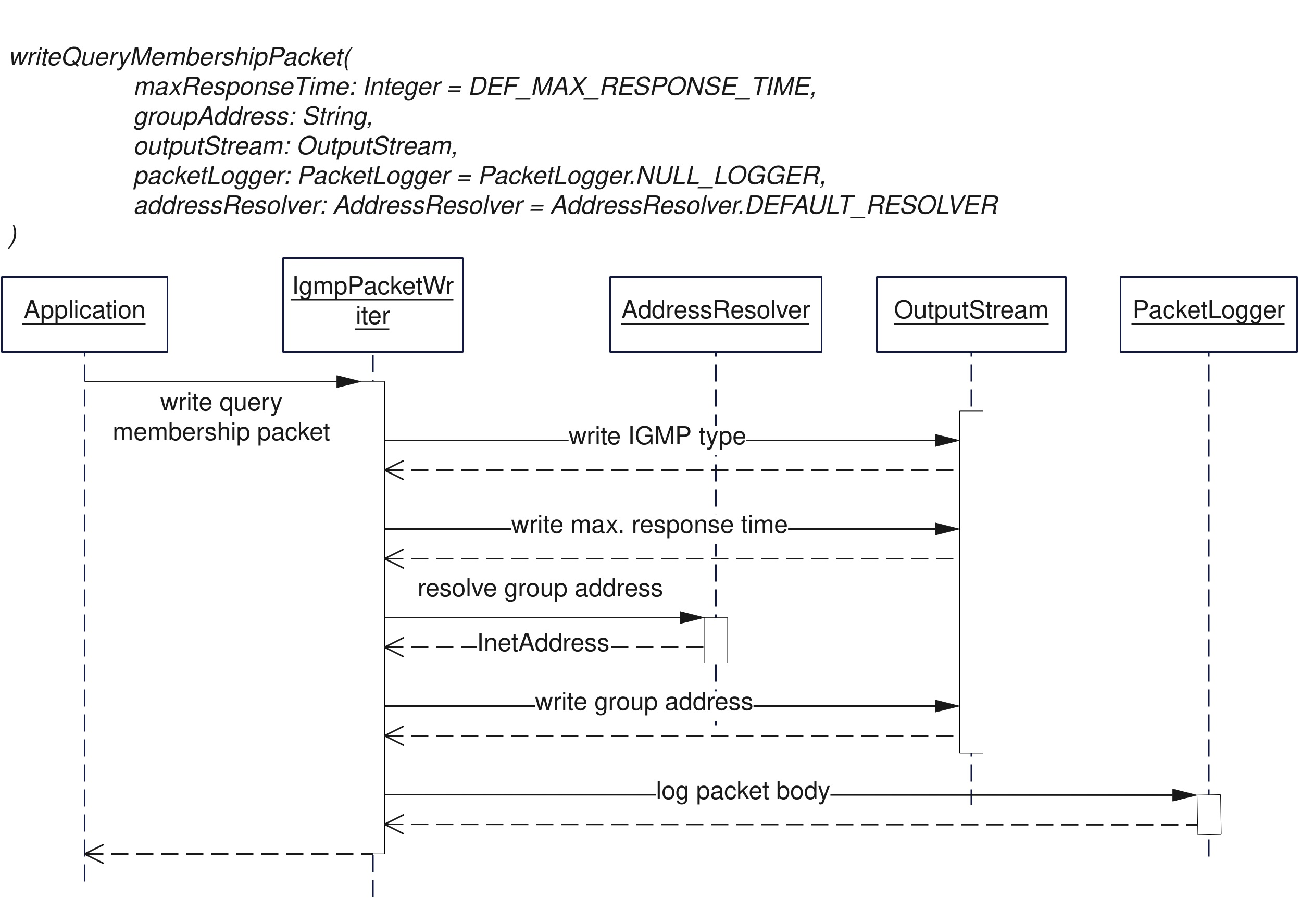
\includegraphics[width=1.0
    \textwidth]{def_specification_of_default_values}
    \caption{Default Values: Specification of default values}
    \label{fig:def_specification_of_default_values}
\end{figure}

\begin{itemize}
    \item \textit{maxResponseTime}:
    This primitive \textit{Integer} type parameter allows direct specification of the default value without the need
    for additional entities.
    \item \textit{packetLogger}:
    This parameter is of type \textit{PacketLogger} which is modeled by another interface.
    The default value of the parameter is set to \textit{PacketLogger.NULL\_LOGGER},
    a constant that follows the Null Object design pattern \cite[Chapter~18]{posa4}.
    Figure~\ref{fig:def_null_logger} demonstrates the implementation of this constant, representing an instance
    of the \textit{PacketLogger} subclass \textit{NullPacketLogger} that does not log anything, merely ignoring
    all input calls.
    This implementation mitigates the need to handle null references in the \textit{writeQueryMembershipPacket} method.
    \item \textit{addressResolver}:
    The parameter, of type \textit{AddressResolver}, adheres to a distinct interface.
    The default value is set to \textit{AddressResolver.DEFAULT\_RESOLVER}, a constant representing an instance
    of a dummy subclass of the \textit{AddressResolver} interface.
    The implementation of this subclass does not attempt to resolve the address and only returns the input address
    if it matches the pattern of an IP address.
    Figure~\ref{fig:def_default_address_resolver} provides view on implementation of the constant,
    which is more complex than the Null Object design pattern, featuring at least simple pattern-matching logic.
\end{itemize}

\begin{figure}[!htb]
    \centering
    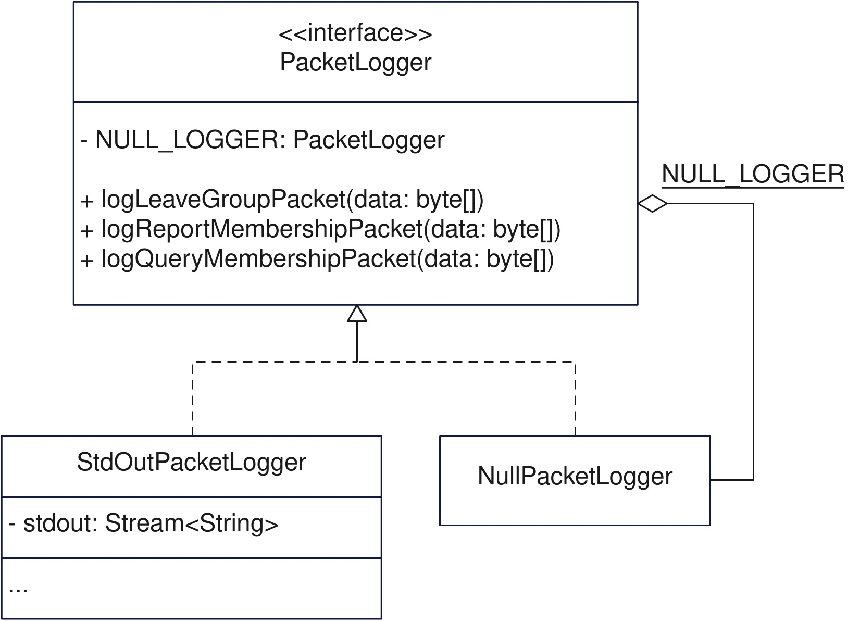
\includegraphics[width=0.66
    \textwidth]{def_null_logger}
    \caption{Default Values: Null logger}
    \label{fig:def_null_logger}
\end{figure}

\begin{figure}[!htb]
    \centering
    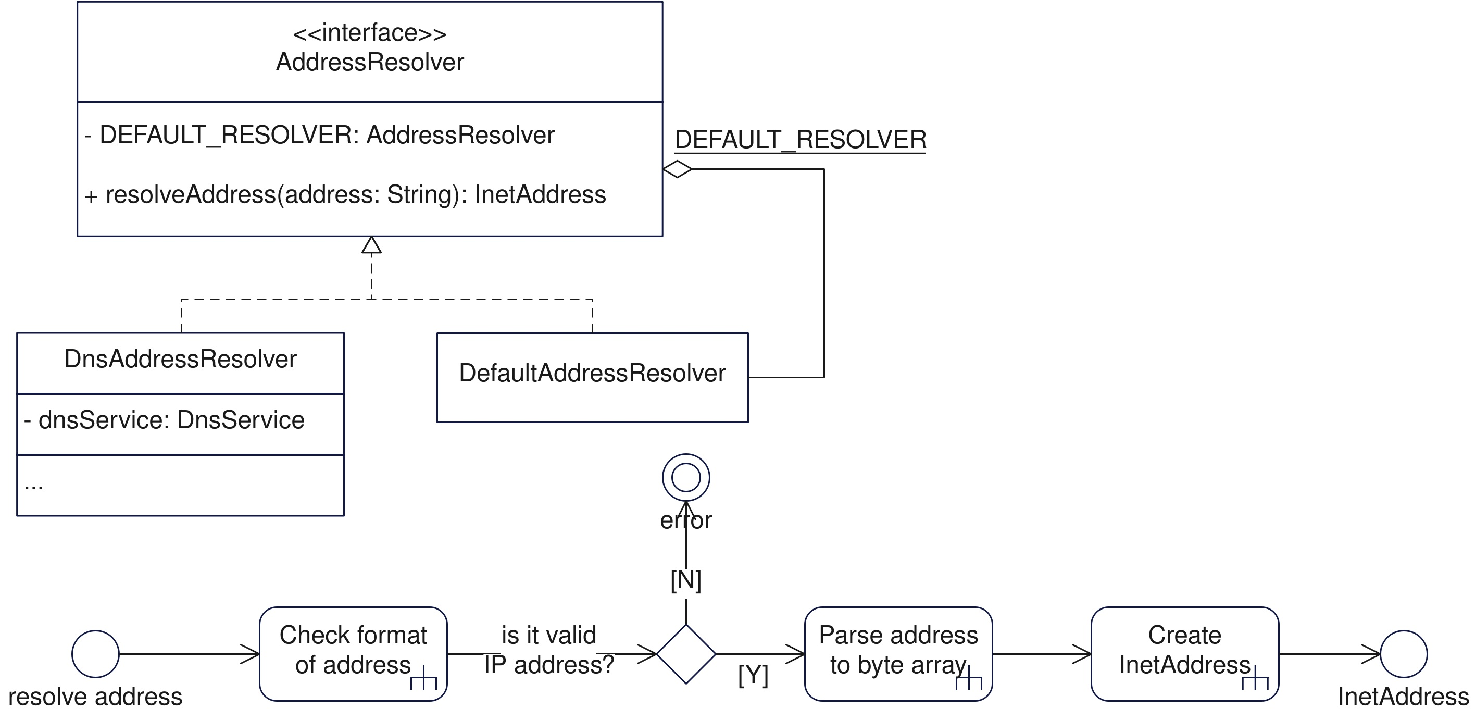
\includegraphics[width=1.0
    \textwidth]{def_default_address_resolver}
    \caption{Default Values: Default address resolver}
    \label{fig:def_default_address_resolver}
\end{figure}

Benefits of the Default Values approach:

\begin{itemize}
    \item Improved readability of method signature:
    The method signature becomes more readable, making it clear which parameters are optional and the values
    used if not specified by the caller.
    The method definition serves as documentation, enhancing code clarity.
    \item Removal of null reference handling in implementation:
    By separating concerns, the handling of null references or values in the implementation of the interface method
    is eliminated.
    This often involves repetitive conditional statements checking whether a parameter is null or not,
    resulting in more readable and maintainable code.
\end{itemize}

Drawbacks of the Default Values approach:

\begin{itemize}
    \item Limited flexibility:
    Default values are static and cannot be changed at runtime.
    This limitation can impact the flexibility of the code, especially if there is a need to alter these values
    based on specific conditions or configurations.
    \item Challenges with complex types:
    For some complex types, creating a default implementation may not always be feasible.
    If a type defines a method that returns a value of a certain type, mocking the return type becomes necessary.
    Additionally, in some languages, a type or method can be marked as final, preventing the creation of subclasses
    or the override of specific method implementations.
    If the type is defined in an external library, updating its constraints is challenging.
\end{itemize}

Common use-cases of the Default Values approach:

\begin{itemize}
    \item Specification of default values for infrequently used parameters:
    The Default Values approach is useful for specifying default values for optional parameters that are not frequently
    used by clients deployed in a production environment.
    These parameters might be utilized in debugging modes or testing environments.
    \item Avoiding extensive overloading of method signatures:
    It helps in decreasing the impact of the API Rooting issue by avoiding extensive overloading
    of the method signature.
    In scenarios with numerous optional parameters, creating all possible combinations of methods becomes impractical.
    Additional interface methods could significantly increase maintenance costs.
\end{itemize}
